% AE646 research poster, A0 portrait (841 x 1189 mm). Build: cd poster && tectonic PINNacles_AE646_Poster.tex
% Figures: poster/figs (python3 poster/make_figs.py) and stage3/figures (report figures).
\documentclass{article}
\usepackage[paperwidth=841mm,paperheight=1189mm,margin=20mm]{geometry}
\usepackage{fontspec}
\setmainfont{texgyreheros}[Extension=.otf, UprightFont=*-regular, BoldFont=*-bold, ItalicFont=*-italic, BoldItalicFont=*-bolditalic]
\usepackage{unicode-math}
\setmathfont{texgyrepagella-math.otf}
\usepackage{graphicx,xcolor,booktabs,array,tabularx,enumitem}
\usepackage[most]{tcolorbox}
\graphicspath{{figs/}{../stage3/figures/}}
\pagestyle{empty}
\setlength{\parindent}{0pt}
\setlength{\parskip}{0.45em}

\definecolor{navy}{HTML}{142F4E}
\definecolor{blue}{HTML}{2F7FD1}
\definecolor{green}{HTML}{1E8E5A}
\definecolor{orange}{HTML}{C96F1E}
\definecolor{grey}{HTML}{5F6B7A}
\definecolor{pale}{HTML}{F2F6FB}
\definecolor{cream}{HTML}{FFF8F0}

\newcommand{\body}{\fontsize{23}{29}\selectfont}
\newcommand{\smalltext}{\fontsize{20}{24}\selectfont}
\newtcolorbox{psec}[2][blue]{enhanced, breakable=false, colback=white, colframe=#1, boxrule=1.6mm, arc=5mm,
  left=7mm, right=7mm, top=4mm, bottom=4mm, title={#2}, coltitle=white, colbacktitle=#1,
  fonttitle=\bfseries\fontsize{33}{39}\selectfont, toptitle=2.5mm, bottomtitle=2.5mm, before skip=0mm, after skip=9mm}
\newtcolorbox{keybox}[1][orange]{enhanced, colback=cream, colframe=#1, boxrule=1mm, arc=4mm, left=6mm, right=6mm, top=3mm, bottom=3mm,
  fontupper=\bfseries\color{#1}\fontsize{23}{28}\selectfont, halign=center, before skip=4mm, after skip=2mm}
\newcommand{\stat}[3]{\begin{tcolorbox}[enhanced, colback=pale, colframe=pale, arc=4mm, left=3mm, right=3mm, top=3mm, bottom=3mm, halign=center, nobeforeafter, width=#1]
  {\bfseries\color{green}\fontsize{50}{56}\selectfont #2}\\[2mm]{\color{grey}\fontsize{20}{24}\selectfont #3}\end{tcolorbox}}
\setlist[itemize]{leftmargin=1.1em, itemsep=0.25em, topsep=0.2em, label={\color{blue}\textbullet}}

\begin{document}
\body
% ------------------------------------------------------------------ header
\begin{tcolorbox}[enhanced, colback=navy, colframe=navy, arc=0mm, left=18mm, right=18mm, top=14mm, bottom=12mm, after skip=12mm]
\color{white}
{\bfseries\fontsize{86}{98}\selectfont Fourier Neural Operators for Parametric Darcy Flow:\\ What Really Drives Accuracy}\par\vspace{8mm}
{\fontsize{40}{48}\selectfont Aryamann Srivastava, Varun Sathaye, Atishay Jain, Vedant S.\ Tiwari \quad\textbar\quad Team PINNacles}\par\vspace{4mm}
{\fontsize{30}{36}\selectfont\color{white!80!blue} Department of Aerospace Engineering, IIT Kanpur \quad\textbar\quad AE646: Scientific Machine Learning for Fluid Mechanics \quad\textbar\quad November 2026}
\end{tcolorbox}

% ------------------------------------------------------------------ key numbers strip
\stat{0.235\linewidth}{0.0202}{final FNO test error (MLP: 0.0415)}\hfill
\stat{0.235\linewidth}{2\,$\times$ / 10\,$\times$}{more accurate / fewer parameters than the MLP}\hfill
\stat{0.235\linewidth}{0.052 $\to$ 0.025}{error halved by the training recipe alone}\hfill
\stat{0.235\linewidth}{5--35\,$\times$}{faster than a finite-volume solver (GPU)}
\vspace{10mm}

% ------------------------------------------------------------------ three columns
\begin{minipage}[t]{0.322\linewidth}\vspace{0pt}
\begin{psec}{1\quad Problem and data}
Steady flow in a porous medium: predict the pressure $u$ from the permeability map $\kappa$,
\[ -\nabla\cdot\big(\kappa\,\nabla u\big)=1 \ \text{ in } (0,1)^2,\qquad u=0 \text{ on the boundary}, \]
with $\kappa\in\{0.1,\,1.0\}$ (thresholded random field). We learn the \textbf{operator} $\mathcal G:\kappa\mapsto u$, so a new map is answered in one forward pass, without a solve.
\begin{itemize}
\item \textbf{Data:} PDEBench 2D Darcy ($\beta=1$), 10,000 real solver outputs at $128^2$, subsampled to $64^2$.
\item \textbf{Split} (fixed, seed 42): 900 train, 100 validation, 200 test. All choices on validation, test used once.
\item \textbf{Inputs:} $\kappa$ plus $x,y$ coordinates; standardised with training statistics.
\end{itemize}
{\smalltext\color{grey} Example predictions (best, typical, worst) are in panel 5.}
\end{psec}

\begin{psec}{2\quad Two models, same inputs}
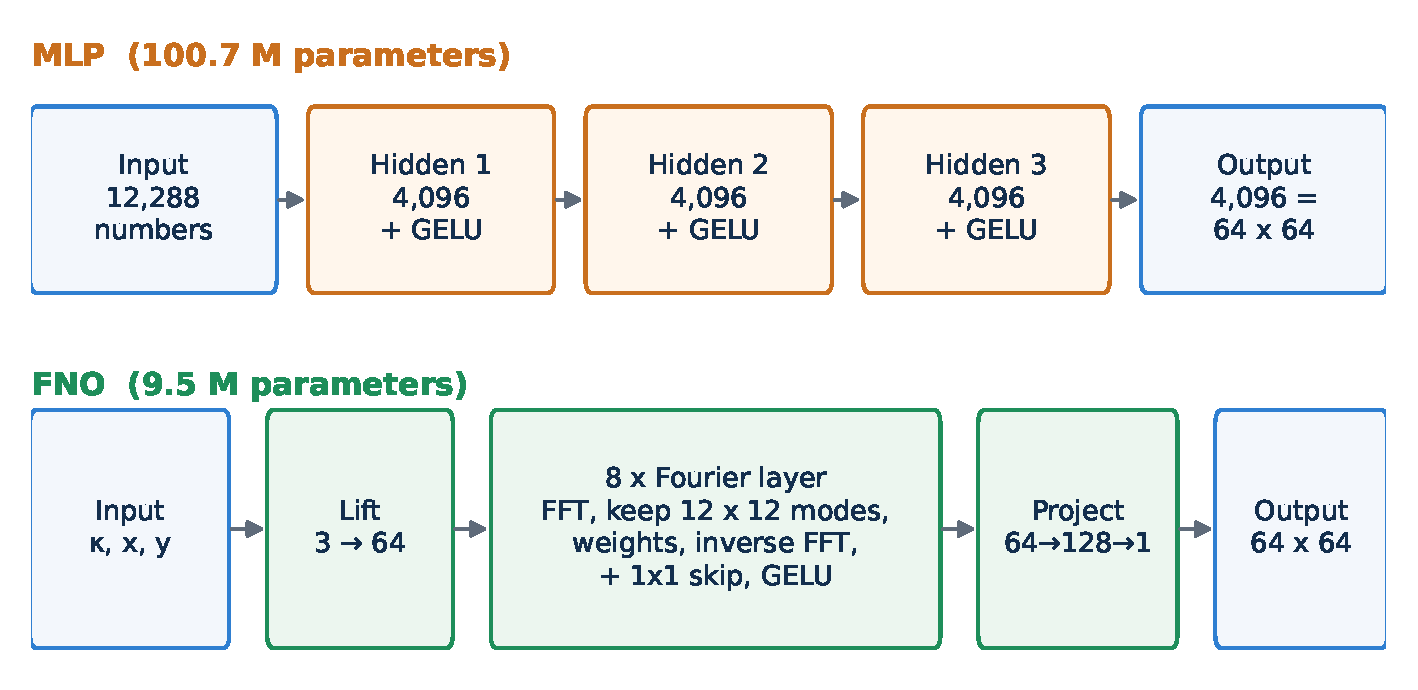
\includegraphics[width=\linewidth]{fig_poster_models.pdf}
\begin{itemize}
\item \textbf{MLP:} flattens the grid into 12,288 numbers. No notion of neighbouring pixels. 100.7\,M parameters.
\item \textbf{FNO:} each Fourier layer transforms to frequencies, keeps the lowest $12\times12$ modes, mixes channels with learned complex weights $R(k)$, transforms back and adds a local path:
\[ v_{\ell+1}=\sigma\big(W v_\ell+\mathcal F^{-1}[\,R\cdot\mathcal F(v_\ell)\,]\big). \]
By the convolution theorem this is a global convolution at $O(N\log N)$ cost. 9.5\,M parameters.
\end{itemize}
\end{psec}

\begin{psec}{3\quad Training and metric}
Per-sample relative $L_2$ error in physical units, with pixel sums ($j$) taken separately in numerator and denominator; the loss averages it over a batch of $B=16$ maps:
\[ \mathcal L=\frac{1}{B}\sum_{i=1}^{B}\frac{\sqrt{\sum_j(\hat u_{ij}-u_{ij})^2}}{\sqrt{\sum_j u_{ij}^2}} \]
\begin{itemize}
\item AdamW, learning rate $10^{-3}$, weight decay $10^{-4}$, one cosine decay.
\item \textbf{D4 augmentation:} the PDE is exactly symmetric under the 8 rotations/flips of the square, applied at $128^2$ before subsampling.
\item Studies: 5,700 to 20,000 steps. Final models: 60,000 steps, 5 seeds.
\end{itemize}
\end{psec}

\begin{psec}[green]{4\quad Final models}
\centering
{\renewcommand{\arraystretch}{1.25}
\begin{tabular}{@{}lccc@{}}\toprule
Model & Params & Mean error & Median\\\midrule
FNO & 9.5\,M & $\mathbf{0.0202\pm0.0004}$ & 0.0070\\
MLP & 100.7\,M & $0.0415\pm0.0009$ & 0.0272\\\bottomrule
\end{tabular}}\par\vspace{2mm}
\raggedright FNO: 12 modes, width 64, 8 layers. MLP: $3\times4096$, tuned on validation. 5 seeds, 60,000 steps. The FNO lead grew from $1.6\times$ (Stage 2) to $2\times$ once both models were trained well.
\end{psec}

\begin{psec}{5\quad Example test predictions}
\begin{center}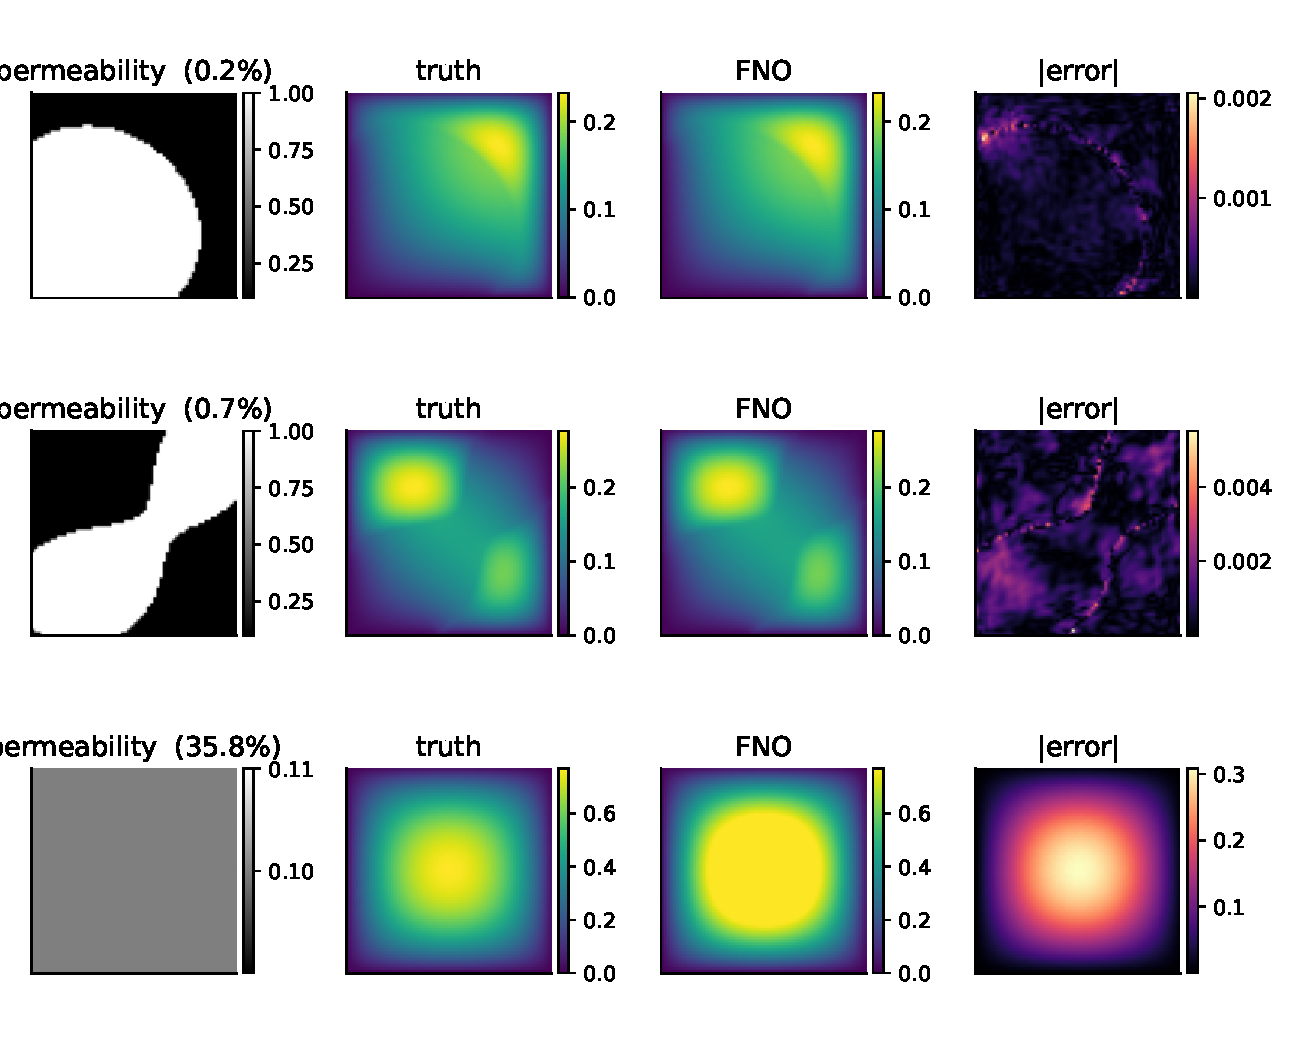
\includegraphics[width=0.84\linewidth]{fig_poster_samples.pdf}\end{center}
{\smalltext\color{grey} Best (0.2\,\%), typical (0.7\,\%) and worst (36\,\%) test maps of the final FNO: permeability, truth, prediction, error. The worst map has uniform $\kappa=0.1$: right shape, wrong height.}
\end{psec}

\end{minipage}\hfill
%
\begin{minipage}[t]{0.322\linewidth}\vspace{0pt}
\begin{psec}{6\quad Finding 1: the training recipe}
Stage 2 trained on MSE (the metric is relative), restarted the learning rate every 200 steps and used no augmentation. Fixing all three, same model and budget (3 seeds):
\begin{center}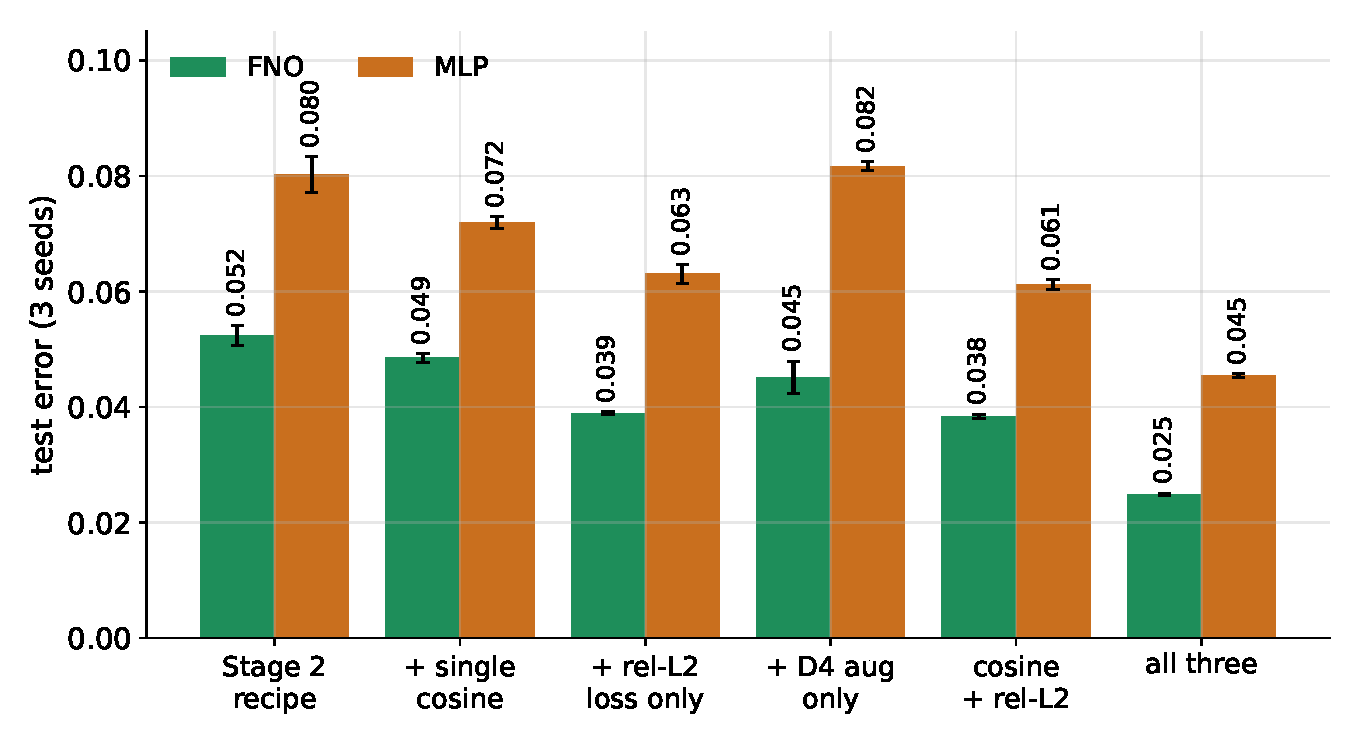
\includegraphics[width=0.96\linewidth]{fig_poster_recipe_ablation.pdf}\end{center}
\begin{keybox}Same model: FNO 0.052 $\to$ 0.025, MLP 0.080 $\to$ 0.045\end{keybox}
\end{psec}

\begin{psec}{7\quad Finding 2: architecture matters little}
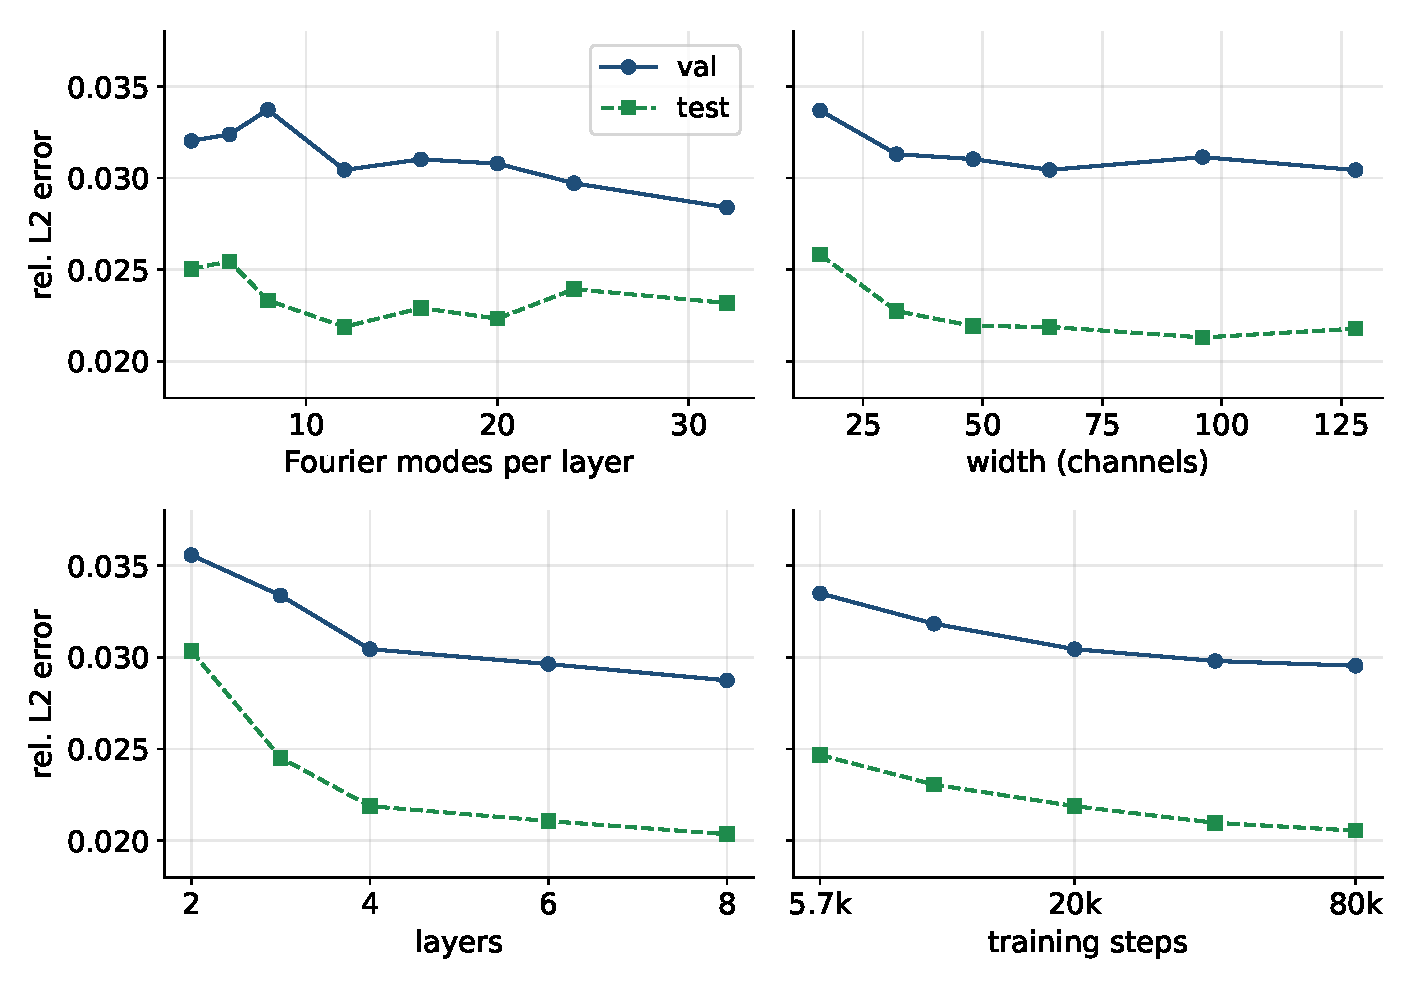
\includegraphics[width=\linewidth]{fig_poster_arch.pdf}
\begin{itemize}
\item Modes 4 to 32 and width $\ge32$: nearly flat. Depth 2 $\to$ 8 layers: 0.030 $\to$ 0.020.
\item Batch 8/16/32: 0.0222 / 0.0219 / 0.0221. Learning rate $5\cdot10^{-4}$ to $2\cdot10^{-3}$: within 0.001.
\item 12 modes chosen on validation: 32 modes cost $7\times$ the parameters and run $3.6\times$ slower for no gain.
\end{itemize}
\end{psec}

\begin{psec}{8\quad Why the MLP cannot catch up}
\begin{center}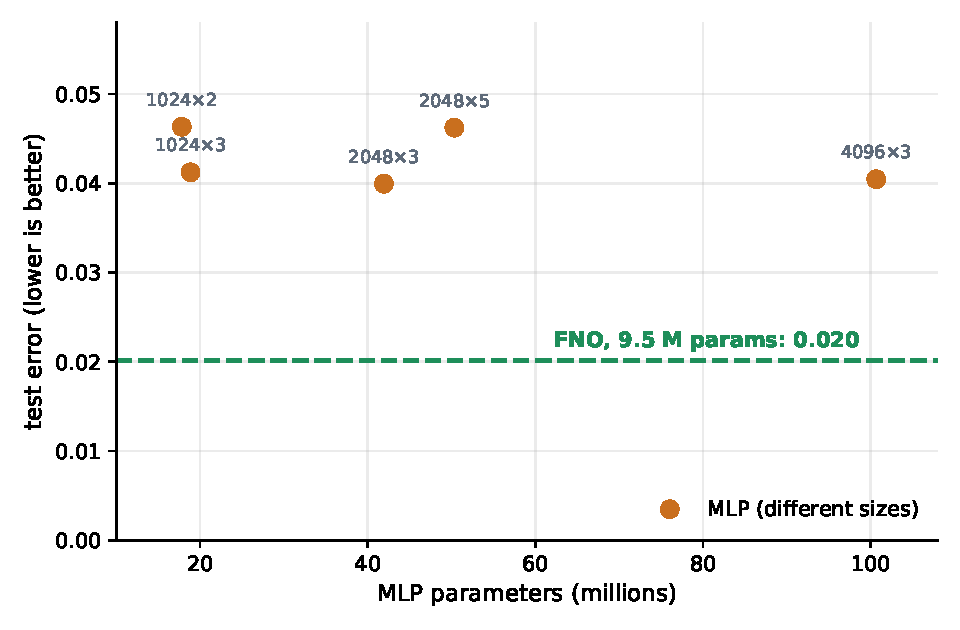
\includegraphics[width=0.88\linewidth]{fig_deck_mlp_limit.pdf}\end{center}
$10\times$ more parameters, 3$\times$ more steps or 10$\times$ more data leave the MLP near 0.035 to 0.046. An FNO trained on only \textbf{400} maps (0.026) beats an MLP trained on \textbf{9,700} (0.036). Likely reason (not tested): without spatial structure it must relearn the same local physics at every pixel.
\end{psec}

\begin{psec}{9\quad Data and resolution}
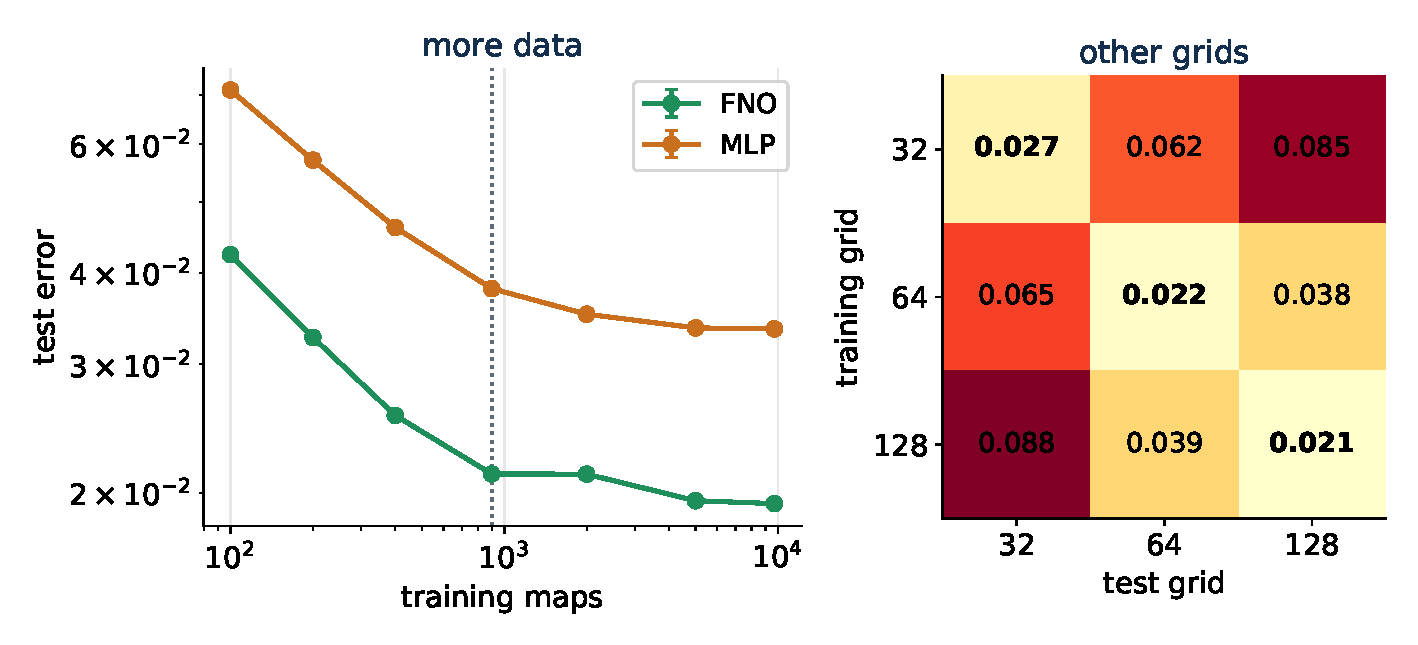
\includegraphics[width=\linewidth]{fig_poster_data.pdf}
\begin{itemize}
\item FNO error: 100 maps 0.044, 400 maps 0.026, 900 maps 0.022, 5,000 maps 0.020; levels off near 0.02.
\item Same-grid error at $32^2/64^2/128^2$: 0.027 / 0.022 / 0.021. A $64^2$ model is 2 to 3$\times$ worse on another grid.
\end{itemize}
\end{psec}
\end{minipage}\hfill
%
\begin{minipage}[t]{0.322\linewidth}\vspace{0pt}
\begin{psec}{10\quad FNO versus a classical solver}
Our cell-centred finite-volume solver: a water balance in every cell, face permeability by harmonic mean, one sparse system $Au=b$ solved by sparse LU, boundary treatment calibrated on validation data.
\begin{center}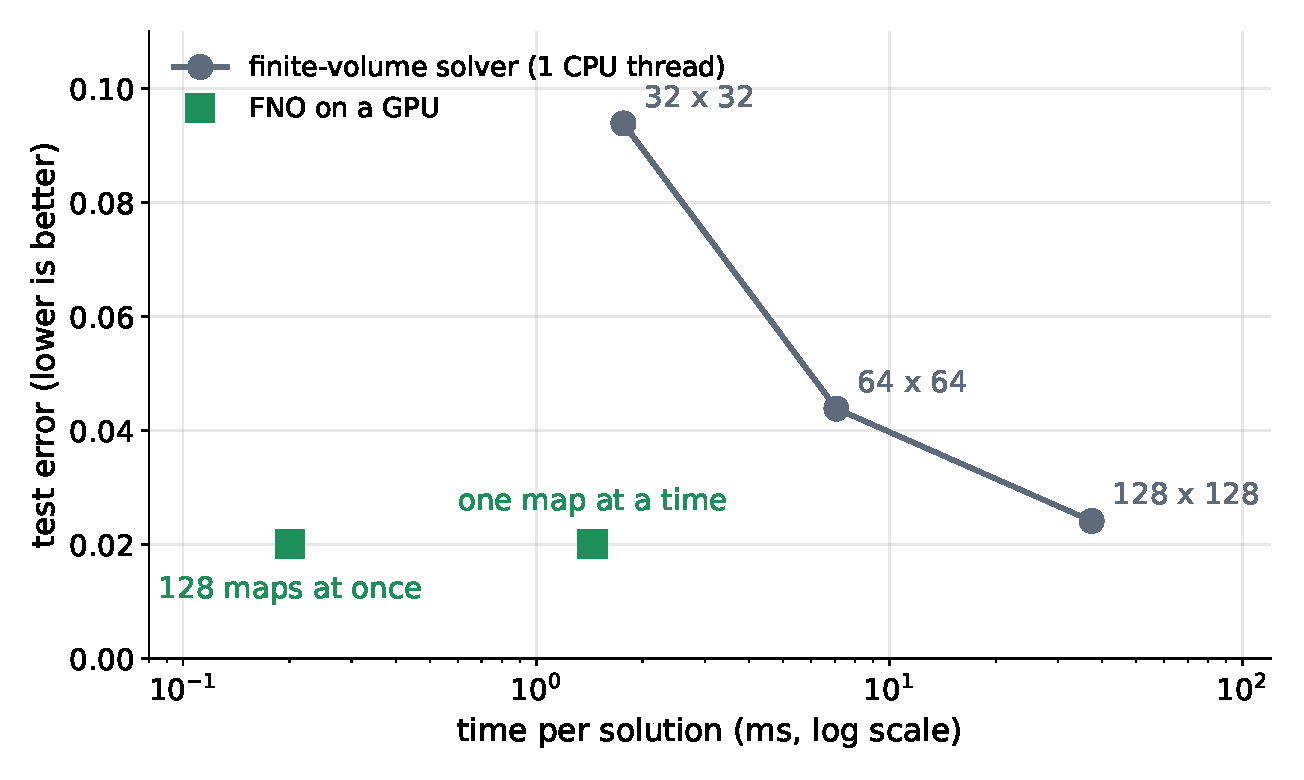
\includegraphics[width=0.92\linewidth]{fig_poster_solver.pdf}\end{center}
\begin{itemize}
\item At $64^2$: FNO error \textbf{0.020} vs solver 0.044; solver 7.1\,ms per map (one CPU thread).
\item FNO on a GPU: 1.4\,ms per map, 0.2\,ms per map in batches of 128, i.e.\ \textbf{5--35$\times$ faster}.
\item On one CPU core the solver is faster (7 vs 37\,ms); training pays off after about $5\times10^4$ solves.
\end{itemize}
\end{psec}

\begin{psec}{11\quad Does it obey the physics?}
\begin{center}
\begin{tabular}{@{}ccc@{}}
{\bfseries\color{green}\fontsize{40}{46}\selectfont 0.1157} & {\bfseries\color{green}\fontsize{40}{46}\selectfont 1.7\,\%} & {\bfseries\color{green}\fontsize{40}{46}\selectfont 0.0015\,\%}\\
{\smalltext\color{grey} edge level (truth 0.1159)} & {\smalltext\color{grey} error in mean pressure} & {\smalltext\color{grey} pixels below zero}
\end{tabular}
\end{center}
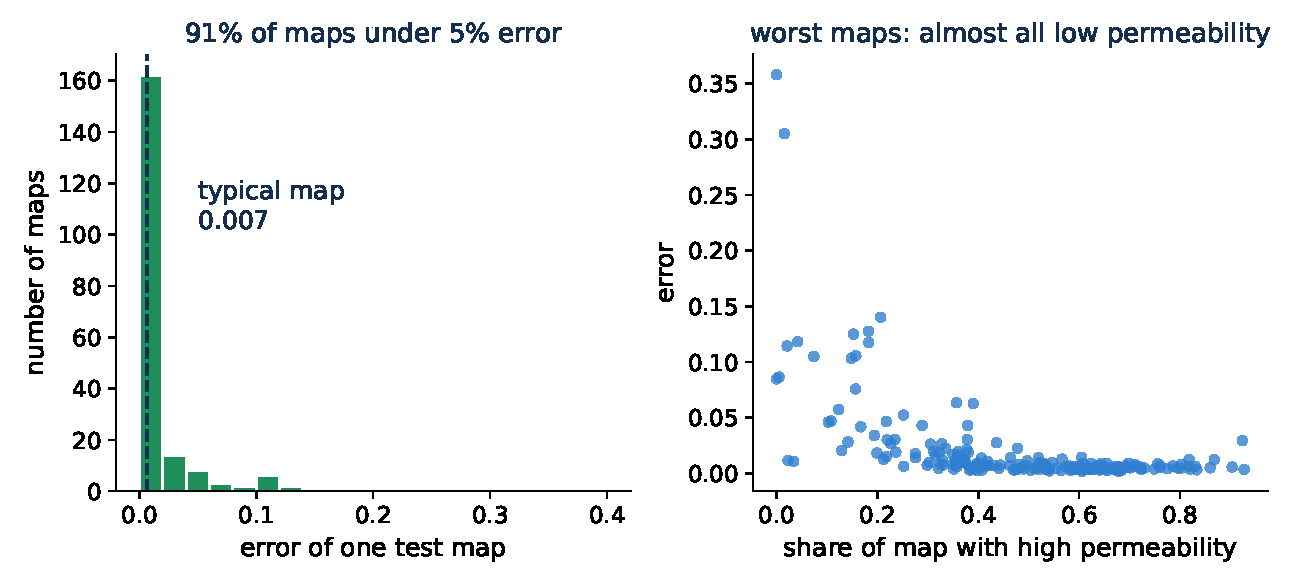
\includegraphics[width=\linewidth]{fig_poster_physics.pdf}
91\,\% of test maps are under 5\,\% error. The worst maps are almost entirely low-permeability: tall pressure, rare in training (27 of 900), right shape but wrong height (up to 36\,\%).
\end{psec}

\begin{psec}[orange]{12\quad Robustness (added after review)}
\textbf{Noisy labels.} Gaussian noise (1, 5, 10\,\% of each map) on the training pressure maps, clean test maps:
\begin{center}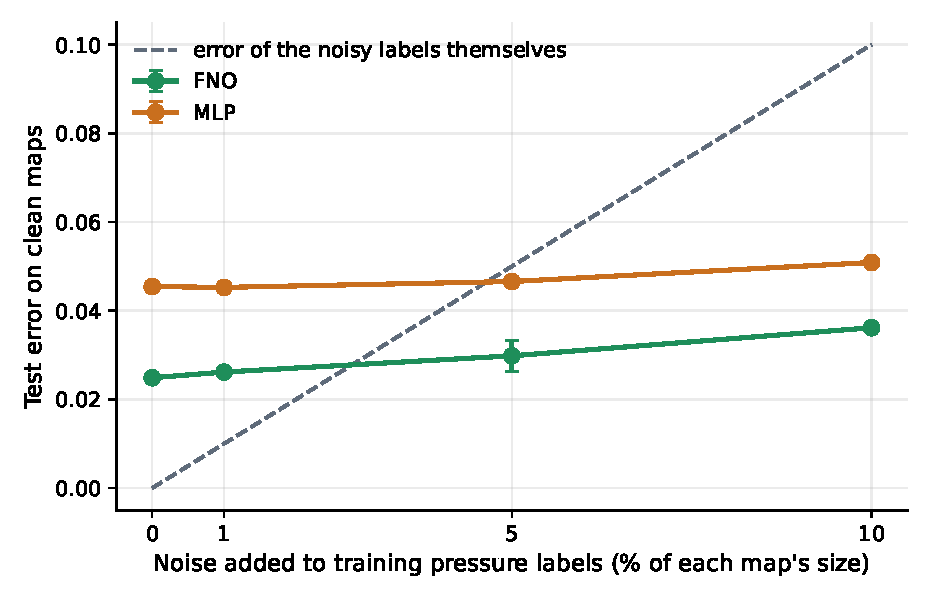
\includegraphics[width=0.8\linewidth]{fig_noise.pdf}\end{center}
At 10\,\% noise: FNO 0.025 $\to$ 0.036, MLP 0.045 $\to$ 0.051. The FNO stays ahead at every level.\par
\textbf{Self-adjusting sample weights.} Each map's weight follows its own running error. It finds the 27 hard training maps (weight $\approx2.7\times$), but their test error does not improve (0.170 vs 0.172) and the overall error rises slightly (0.0249 $\to$ 0.0265): a negative result.
\end{psec}

\begin{psec}[navy]{13\quad Conclusions and limitations}
\begin{itemize}
\item \textbf{Training mattered most:} matching loss and metric, one learning-rate decay and symmetry augmentation halved the error.
\item \textbf{Structure beats size:} the FNO is $2\times$ more accurate than a tuned MLP with $10\times$ fewer parameters, and robust to label noise.
\item \textbf{Limits:} one PDE and dataset; agreement with the data, not the exact PDE; tied to the training grid; speed gain needs a GPU; nearly uniform maps remain hard.
\end{itemize}
{\smalltext\color{grey} Refs: Li et al., FNO, ICLR 2021; Takamoto et al., PDEBench, NeurIPS D\&B 2022. 167 training runs; code, per-run results and notebook in the project repository. AI tools were used for coding and drafting; all numbers come from real runs.}
\end{psec}
\end{minipage}
\end{document}
